\documentclass[11pt,border=5pt]{standalone}
\usepackage{fontspec}
\setmainfont{cmunrm.otf}[BoldFont=cmunbx.otf,ItalicFont=cmunti.otf,BoldItalicFont=cmunbi.otf]
\usepackage{amsmath}
\usepackage{unicode-math}
\setmathfont{NewCMMath-Regular.otf}
\usepackage{tikz}
\usetikzlibrary{arrows.meta,patterns,angles,quotes}
\begin{document}
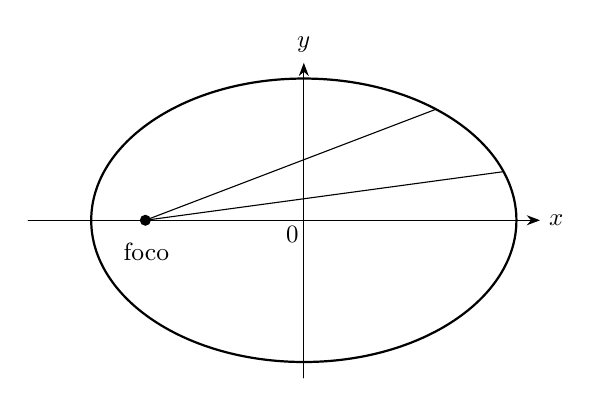
\begin{tikzpicture}[>=Stealth,font=\small,line cap=round,line join=round]
\draw[->,thin] (-3.5,0) -- (3,0) node[right] {$x$};
\draw[->,thin] (0,-2) -- (0,2) node[above] {$y$};
\node at (-0.14,-0.18) {$0$};
\draw[thick] (0,0) ellipse (2.7 and 1.8);\fill (-2.01246,0) circle(2pt);\draw[thin] (-2.01246,0) -- (2.5363063246879234,0.6172160534198124);
\draw[thin] (-2.01246,0) -- (1.6783469143307939,1.4099884373294702);
\node at (-2,-0.4) {foco};

\end{tikzpicture}
\end{document}
